\documentclass[20pt]{article}
\usepackage[utf8]{inputenc}
\usepackage{amsmath}
\usepackage{amssymb}
\usepackage{amsfonts}		 
\usepackage{enumitem}
\usepackage{fancyheadings}
\usepackage{mathtools}
\usepackage{tikz}
\usepackage{fancybox}
\usetikzlibrary{automata,positioning}
\DeclarePairedDelimiter{\ceil}{\lceil}{\rceil}
\DeclarePairedDelimiter\floor{\lfloor}{\rfloor}
\usepackage[margin=3cm]{geometry}
\usepackage{changepage}
\usepackage{listings}

\title{CSC263H1 Homework 3}
\author{Tony Yang, Wendy Guo, Martin Chak}
\date{February 13th 2020}

\begin{document}

%BEGIN TITLE PAGE

\maketitle

%END TITLE PAGE

\newpage

%BEGIN Q1

\noindent
\textbf{Question 1:}\\
\textbf{Done by: Wentao Yang, Martin Chak; Written by: Martin Chak}\\

\noindent
\begin{text}
    a) Insert keys 22, 3, 4, 15, 25, 0, 8, 29, 19, 12, 7, 11 (in this order) into an initially empty AVL tree,and show the resulting AVL tree $T$, including the balance factor of each node (only the final tree should be shown)
\end{text}

\begin{adjustwidth}{-0pt}{-0pt}
\ovalbox{
    \begin{tikzpicture}[level/.style={sibling distance=60mm/#1}]
        \node [circle,draw] (a){$15$}
          child {node [circle,draw] (b) {$4$}
            child {node [circle,draw] (c) {$3$}
              child {node [circle,draw,left=1cm] (d) {$0$}} 
              %child {node [circle,draw] (h) {$1$}}
            }
            child {node [circle,draw] (e) {$8$}
              child {node [circle,draw] (f) {$7$}} 
              child {node [circle,draw] (g) {$12$}
                child {node [circle, draw, right= 0.5cm] (h) {$11$}}}
            }
          }
          child {node [circle,draw] (i) {$22$}
            child {node [circle,draw] (j) {$19$}}
            child {node [circle,draw] (k) {$25$}
              child {node [circle,draw, right=0.5cm] (l) {$29$}}
          }
        };
        
        \path (a) -- (a) node [left=0.5cm, above] {-};
        \path (b) -- (b) node [left=0.5cm, above] {+};
        \path (c) -- (c) node [left=0.5cm, above] {-};
        \path (d) -- (d) node [left=0.5cm, above] {0};
        \path (e) -- (e) node [left=0.5cm, above] {+};
        \path (f) -- (f) node [left=0.5cm, above] {0};
        \path (g) -- (g) node [left=0.5cm, above] {+};
        \path (h) -- (h) node [left=0.5cm, above] {0};
        \path (i) -- (i) node [right=0.5cm, above] {+};
        \path (j) -- (j) node [left=0.5cm, above] {0};
        \path (k) -- (k) node [left=0.5cm, above] {+};
        \path (l) -- (l) node [left=0.5cm, above] {0};
    \end{tikzpicture}
}
\end{adjustwidth}

\noindent
\begin{text}
    \\\\
    b) Remove the node with the value of 19 from the node
\end{text}

\begin{adjustwidth}{-0pt}{-0pt}
\ovalbox{
    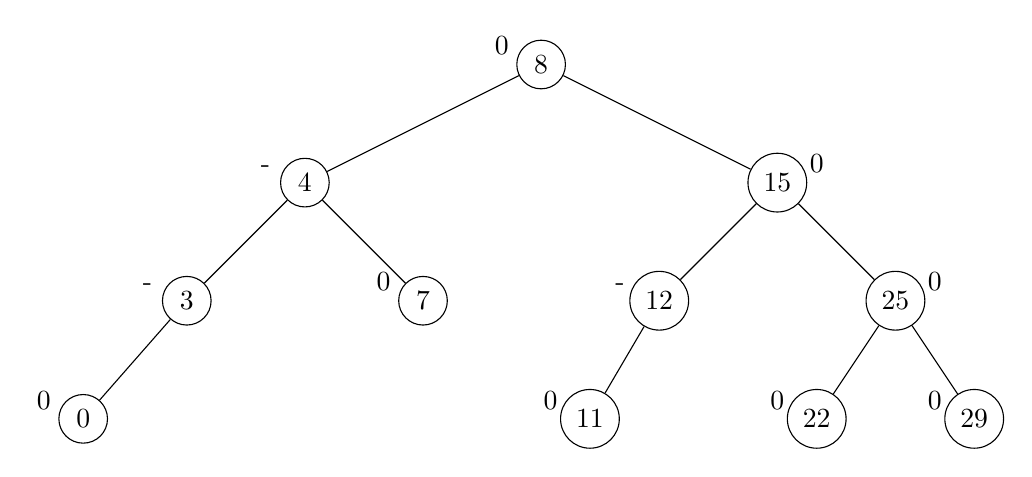
\begin{tikzpicture}[level/.style={sibling distance=60mm/#1}]
        \node [circle,draw] (a){$8$}
          child {node [circle,draw] (b) {$4$}
            child {node [circle,draw] (c) {$3$}
              child {node [circle,draw,left=1cm] (d) {$0$}} 
            }
            child {node [circle,draw] (e) {$7$}}
          }
          child {node [circle,draw] (f) {$15$}
            child {node [circle,draw] (g) {$12$}
              child {node [circle, draw, left=0.5cm] (h) {$11$}}
            }
            child {node [circle,draw] (i) {$25$}
              child {node [circle,draw] (j) {$22$}}
              child {node [circle,draw] (k) {$29$}}
          }
        };
        
        \path (a) -- (a) node [left=0.5cm, above] {0};
        \path (b) -- (b) node [left=0.5cm, above] {-};
        \path (c) -- (c) node [left=0.5cm, above] {-};
        \path (d) -- (d) node [left=0.5cm, above] {0};
        \path (e) -- (e) node [left=0.5cm, above] {0};
        \path (f) -- (f) node [right=0.5cm, above] {0};
        \path (g) -- (g) node [left=0.5cm, above] {-};
        \path (h) -- (h) node [left=0.5cm, above] {0};
        \path (i) -- (i) node [right=0.5cm, above] {0};
        \path (j) -- (j) node [left=0.5cm, above] {0};
        \path (k) -- (k) node [left=0.5cm, above] {0};
    \end{tikzpicture}
}
\end{adjustwidth}

%END Q1

\newpage

%BEGIN Q2

\noindent
\textbf{Question 2:}\\
\textbf{Done by: Martin Chak; Written by: Martin Chak}\\
\noindent
\begin{text}
    Create a data structure that tracks the housing entries which tracks the price of a house and the floor area of the house. The data structure must be an augmented AVL tree such that:
\end{text}
\begin{align*}
    &Insert(D, x): \text{If $x$ is a pointer to a new listing, insert the listing pointed to by $x$ into D.}\\
    &Delete(D, x): \text{If $x$ is a pointer to a listing in D, remove that listing from D.}\\
    &MaxArea(D, p): \text{Return the maximum floor area of listings whose price is at most p, return -1 if none}
\end{align*}
\noindent
\begin{text}
    So our data structure is just an AVL tree sorted by the price of the listing, however it is special since it will also contain a pointer to the listing with the largest floor area in its current tree (which constitutes as itself and its children). For example, the root of the entire AVL tree will contain a pointer that points to the max area for all listings in the entire tree. We can illustrate the data structure with an example below:
\end{text}

\begin{adjustwidth}{50pt}{25pt}
\ovalbox{
    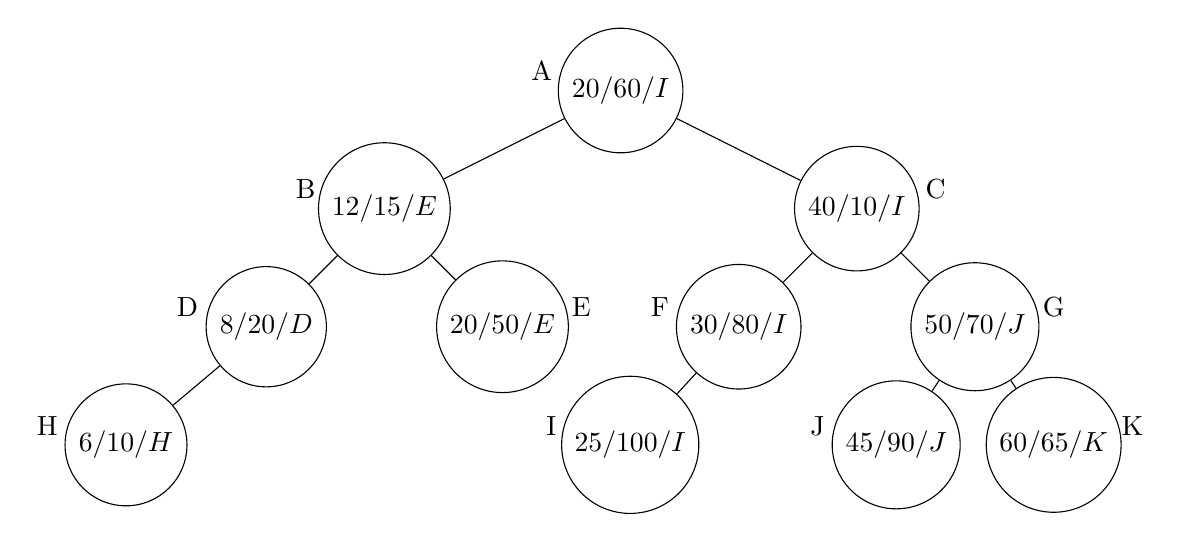
\begin{tikzpicture}[level/.style={sibling distance=60mm/#1}]
        \node [circle,draw] (a){$20/60/I$}
          child {node [circle,draw] (b) {$12/15/E$}
            child {node [circle,draw] (d) {$8/20/D$}
              child {node [circle,draw,left=1cm] (h) {$6/10/H$}} 
            }
            child {node [circle,draw] (e) {$20/50/E$}}
          }
          child {node [circle,draw] (c) {$40/10/I$}
            child {node [circle,draw] (f) {$30/80/I$}
              child {node [circle, draw, left=0.5cm] (i) {$25/100/I$}}
            }
            child {node [circle,draw] (g) {$50/70/J$}
              child {node [circle,draw] (j) {$45/90/J$}}
              child {node [circle,draw] (k) {$60/65/K$}}
          }
        };
        
        \path (a) -- (a) node [left=1cm, above] {A};
        \path (b) -- (b) node [left=1cm, above] {B};
        \path (c) -- (c) node [right=1cm, above] {C};
        \path (d) -- (d) node [left=1cm, above] {D};
        \path (e) -- (e) node [right=1cm, above] {E};
        \path (f) -- (f) node [left=1cm, above] {F};
        \path (g) -- (g) node [right=1cm, above] {G};
        \path (h) -- (h) node [left=1cm, above] {H};
        \path (i) -- (i) node [left=1cm, above] {I};
        \path (j) -- (j) node [left=1cm, above] {J};
        \path (k) -- (k) node [right=1cm, above] {K};
    \end{tikzpicture}
}
\end{adjustwidth}

\noindent
\begin{text}
    So in the above example, each node has a letter that it associates with, annotated on the side of the node. The first number of the node is price, the second is the floor area for the listing, and the letter represents a pointer to the listing with the largest floor area in the sub-tree formed when the node is the root.
\end{text}

\noindent
\begin{text}
    We have outlined our data structure, but we now must show that it can perform the aforementioned operations with $O(log(n))$ time complexity.
    
    \noindent
    \textbf{Insert(D, x)}
    When we insert a new listing, where $x$ is a pointer to the new listing, we insert the node as we would with a normal AVL tree, focusing on properly ordering the prices and then re-balancing the tree. As provided in the lecture and course notes, this will take $O(log(n))$ time. We then need to update the pointers to the node with the largest floor areas, but how long does this take?
    
    \noindent
    We can notice that when we insert a node, only its direct ancestors will need to update their pointers, as only they have changes in their children. This is because rotations and re-insertions are only done on unbalanced trees, and this can only happen to ancestors. Thus after re-balancing, we need to check for the new largest areas in each ancestor sub tree. We can do this by recursively going to each tree and comparing the roots' area with their children's pointers' areas. If one of the children is one of the ancestors, then we continue working on the child until we receive a max pointer from it, this continues until we reach the bottom of the tree which at most will take $O(log(n))$ time.
    
    \noindent
    \textbf{Delete(D, x)}
    When we delete a listing, we re-re-balance the tree by taking the listing with the lowest price that is higher than the removed listing. Then the tree is re-balanced as needed. As provided in the lecture and course notes, this will take $O(log(n))$ time. We will then update the pointers to the node with the largest floor area.
    
    \noindent
    Similarly to the insert algorithm, delete updates the pointers as it would with updating balance factors. We can notice through the notes that when we delete a node, the only nodes that have children who are removed, added, or changed are nodes that lie on the path from the top of the node to the node that is replacing the deleted node (or the deleted node if it is a leaf) on the original pre-deletion tree. Once the tree is rebalanced, we recursively go down to each node and update their max pointers, having them compare the max pointer values of their children and themselves. If a child is a node that also needs to be updated, we go on to update them first, continuing until we reach the bottom of the tree or until the pointer can be properly updated. This will take $O(log(n))$ time which in addition to the time required to delete and rebalance leaves $Delete$ with a $O(log(n))$ time complexity.\\
    
    \noindent
    \textbf{MaxArea(D,p)}
    This algorithm finds the listing with the most floor space given that the price of the listing is at most the given $p$.
    
    \noindent
    Once given the price, we want to go down the tree to find all entries that are less than $p$ and find the max floor space as we come back up. We can write the following program:
\end{text}

\begin{lstlisting}
    def MaxArea(root, price) {
        if (root price is more than price) { #The root is over priced
            if (root.left exists) {
                #Returns an area if left child has roots that work
                #Returns -1 otherwise
                area = MaxArea(root.left, price)
                
                #The right child and the root are overpriced, no need to
                #check them just return the left root area, which could
                #be -1 if there were no viable values
    
                return area
            }
            else {
                return -1
            }
        }
        else { #The root is within the limit
            #Since the root is within the price
            #range, then all its left children are within the range too
            area = -1
            
            if (root.right exists) {
                area = MaxArea(root.right, price)
            }
            
            #Here we compare the left child's max value, 
            #the node and the area and return the max
            #if one of them doesn't exist just remove it from the comparison
            max = max(area, root.left.max, etc.)
            
            return max
        }
    }
\end{lstlisting}
\noindent
\begin{text}
    This goes down into the tree and reaches the bottom, and on the way up, makes comparisons to the max's until we reach the top, taking $log(n)$ steps to traverse down and potentially $3\cdot log(n)$ steps on the way back up, therefore taking $O(log(n))$ time to complete the operation.
\end{text}

%END Q2

\newpage

%BEGIN Q3
\section*{Question 3}
\textbf{Done by: Wendy Guo and Wentao Yang; Written by: Wendy Guo and Wentao Yang}\\
\noindent
\begin{text}
    a) For a given input $d$, the algorithm checks if there exists $x \in X$ and $y \in Y$ such that $d = \sqrt{x^2 + y^2}$ and outputs "YES" or "NO" accordingly. We can iterate through the $n$ values in $Y$, and calculate for each $y \in Y$ a value $k$ such that $k = \sqrt{d^2 - y^2}$. We then hash this value $k$ into a hash table of $n$ buckets at index $\floor{\sqrt{d^2 - y^2}}$. The bucket with index $i$ stores values $[i\cdot\frac{d}{n}, i\cdot\frac{d}{n} + \frac{d}{n})$, using chaining through linked lists to store multiple values. Each $k$ represents a value of x that is a potential solution. Since $k = \sqrt{d^2 - y^2}$, we know its value is always less than $d$, so our range of $[i\cdot\frac{d}{n}, i\cdot\frac{d}{n} + \frac{d}{n})$ will ensure an even distribution of values in the table. \\ \\
    After the $k$ values have been hashed, we can iterate through the values in $X$ to see if any of them exist in the hash table. Due to the way the potential solutions were added, we know that if $x \in X$ is a solution, it will be at index $x\cdot\frac{n}{d}$, which we can calculate in constant time in the hash table. Then we can search through the chained entries at that index to see if there is a match.
\end{text}
\begin{lstlisting}[mathescape=true]
1    Insert($Y$, $d$, table): 
2    for $y$ in $Y$: 
3        table[$\floor{\sqrt{d^2 - y^2}}$] = ($\sqrt{d^2 - y^2}$)
4        
5    Search($X$, table)
6    int n = len(X) # constant time
7    for $x$ in $X$:
8        if $x$ in table[$x\cdot\frac{n}{d}$]:
9            return "YES"
10   return "NO"
\end{lstlisting}
\noindent
\begin{text}
    b) The insert function would take $n$ steps since we perform one insertion per value in $Y$. By SUHA, each of the $n$ buckets will contain one value (keys were distributed evenly). When running Search to iterate through $X$, we iterate through the loop a maximum of $n$ times, while checking whether or not the value $x$ exists in a bucket of the hash table takes constant time. Thus, assuming that the values are hashed into the table evenly, the algorithm takes a total of 2n steps, so the expected run time is $O(n)$. \\
    
    c) If there is no solution, the Search function will have to iterate through all $n$ values in $X$. In addition, if all the values in $Y$ were hashed to the same bucket, they would all be in a linked list of length $n$. Then, there would be $n$ loop iterations of searching through a linked list of length $n$. This in turn would result in $n^2$ steps, so the worst case is $\Theta(n^2)$.
    
\end{text}


%END Q3

\end{document}